\documentclass[a4paper, 12pt, twoside]{article}
\usepackage{estilo}

% ── Margens laterais estritamente oficiais (2.5cm) conforme edital EU ──
\geometry{
  a4paper,
  inner=2.5cm, outer=2.5cm,
  top=2.0cm, bottom=1.5cm,
  headheight=40pt, headsep=12pt
}
\setstretch{0.86}
\setlength{\parindent}{0.70cm}
\setlength{\textfloatsep}{2pt plus 1pt minus 1pt}
\setlength{\intextsep}{2pt plus 1pt minus 1pt}
\setlength{\abovecaptionskip}{1.5pt}
\setlength{\belowcaptionskip}{1.5pt}

\title{Redes Neurais Informadas por Física para Resolução Numérica das Equações Bidimensionais do Calor e de Burgers}

\author{%
  Autor Principal\authorinfo{autor@alu.ufc.br} \\
  Orientador\authorinfo{orientador@ufc.br}
}
\date{}

\begin{document}
\maketitle

%%%%%%%%%%%%%%%%%%%%% RESUMO E ABSTRACT %%%%%%%%%%%%%%%%%%%%%%%%%%%%%%

\qabstract{Resumo}{Palavras-chave}{ODS}{%
A simulação computacional de sistemas físicos governados por Equações Diferenciais Parciais (EDPs) bidimensionais fundamenta a engenharia térmica e a fluidodinâmica. Esquemas clássicos de malha, como o Método de Diferenças Finitas (MDF) formalizado por \textcite{pereira2019}, enfrentam restrições de estabilidade (CFL) e elevado custo na discretização de geometrias complexas. Este trabalho investiga as Redes Neurais Informadas por Física (PINNs) como um paradigma contínuo e livre de malha (\textit{meshless}) na resolução de dois problemas canônicos: a Equação do Calor 2D transiente linear ($\alpha = 0{,}1$) e a Equação de Burgers 2D viscosa ($\nu = 0{,}01$) sob condição inicial quadrupolar com quatro vórtices gaussianos convergentes. As leis de conservação física são integradas ao funcional de perda multiobjetivo via diferenciação automática (\textit{autograd}) e retropropagadas para otimização dos pesos via Adam. Após 20.000 épocas, a PINN atinge resíduo $\mathcal{L}_{\mathrm{total}} = 7{,}95 \times 10^{-5}$ no calor (erro relativo $\epsilon_{L^2} = 1{,}40 \times 10^{-3}$ ou $0{,}14\%$ frente à solução analítica) e $\mathcal{L}_{\mathrm{total}} = 1{,}04 \times 10^{-3}$ em Burgers ($\mathcal{L}_{\mathrm{bc}} = 2{,}31 \times 10^{-6}$), capturando fielmente a dinâmica quadrupolar sem necessidade de malha.%
}{%
redes neurais informadas por física; equação do calor; equação de burgers; equações diferenciais parciais; diferenciação automática%
}{%
indústria, inovação e infraestrutura%
}

\qabstract{Abstract}{Keywords}{SDG}{%
Computational simulation of physical systems governed by two-dimensional Partial Differential Equations (PDEs) is fundamental to thermal engineering and fluid dynamics. Classical mesh-based schemes, such as the Finite Difference Method (FDM) formalized by \textcite{pereira2019}, face strict stability constraints (CFL) and high meshing overhead in complex geometries. This work investigates Physics-Informed Neural Networks (PINNs) as a continuous, mesh-free solver for two canonical problems: the linear transient 2D Heat Equation ($\alpha = 0.1$) and the nonlinear viscous 2D Burgers Equation ($\nu = 0.01$) under a quadrupolar initial condition with four converging Gaussian vortices. Physical conservation laws are directly embedded into a multi-objective loss function via automatic differentiation (\textit{autograd}) and backpropagated for weight optimization using the Adam algorithm. After 20,000 epochs, the PINN achieves residuals of $\mathcal{L}_{\mathrm{total}} = 7.95 \times 10^{-5}$ for heat (relative error $\epsilon_{L^2} = 1.40 \times 10^{-3}$ or $0.14\%$ against analytical solution) and $\mathcal{L}_{\mathrm{total}} = 1.04 \times 10^{-3}$ for Burgers ($\mathcal{L}_{\mathrm{bc}} = 2.31 \times 10^{-6}$), accurately capturing quadrupolar dynamics without meshing.%
}{%
physics-informed neural networks; heat equation; Burgers equation; partial differential equations; automatic differentiation%
}{%
industry, innovation and infrastructure%
}

%%%%%%%%%%%%%%%%%%%%%%%%%%%%%% SEÇÕES %%%%%%%%%%%%%%%%%%%%%%%%%%%%%

\section{Introdução}

A modelagem quantitativa de fenômenos de transporte térmico e dinâmica de fluidos descritos por \textbf{Equações Diferenciais Parciais (EDPs)} é indispensável no projeto de engenharia. Tradicionalmente, esquemas baseados em malha --- como o \textbf{Método de Diferenças Finitas (MDF)}, Elementos Finitos (MEF) e Volumes Finitos (MVF) --- transformam operadores diferenciais contínuos em sistemas algébricos via discretização nodal \parencite{pereira2019}. Em equações não lineares parabólicas e hiperbólicas, conforme formalizado por \textcite{pereira2019}, o MDF requer esquemas implícitos como o método ADI \parencite{peaceman1955adi} para mitigar restrições severas de estabilidade temporal ($\text{CFL} \le 1/2$), demandando malhas estruturadas e acumulando erros de truncamento local $\mathcal{O}(\Delta x^2 + \Delta t^2)$ ao longo da marcha causal.

Em contrapartida, as \textbf{Redes Neurais Informadas por Física (PINNs)}, introduzidas por \textcite{raissi2019pinns}, estabelecem uma abordagem contínua e livre de malha (\textit{meshless}). A solução $u_\theta(\mathbf{x}, t)$ é parametrizada por um Perceptron Multicamadas (MLP) profundo, e os operadores diferenciais são avaliados exatamente no espaço contínuo por \textbf{diferenciação automática (\textit{autograd})}. As leis físicas e condições de fronteira compõem a função de perda multiobjetivo, contornando a discretização nodal e viabilizando inferências instantâneas $\mathcal{O}(1)$.

Este trabalho investiga o arcabouço PINN na resolução de duas EDPs canônicas 2D: (\textit{i}) a \textbf{Equação do Calor 2D} transiente linear, validada quantitativamente frente à Série de Fourier; e (\textit{ii}) a \textbf{Equação vetorial de Burgers 2D Viscosa} sob condição inicial quadrupolar \parencite{burgers1948model, pereira2019}. Analisam-se a dinâmica de perdas, a topologia de fluxos e os ganhos de inferência contínua.

\section{Desenvolvimento}

\subsection{Fundamentação Teórica}

\textbf{1. Equação do Calor 2D:} A condução térmica em sólido homogêneo $\Omega = [0, 1]^2$ com difusividade $\alpha = 0{,}1\,\text{m}^2/\text{s}$ no intervalo $t \in (0, 1{,}0]\,\text{s}$ é regida por:
\begin{equation}
    \mathcal{R}_{\text{calor}}[u] := \frac{\partial u}{\partial t} - \alpha \left( \frac{\partial^2 u}{\partial x^2} + \frac{\partial^2 u}{\partial y^2} \right) = 0, \quad \forall (x, y, t) \in \Omega \times (0, 1{,}0], \label{eq:heat}
\end{equation}
sob repouso inicial $u(x, y, 0) = 0{,}0$ e contorno externo $u|_{\partial\Omega} = 1{,}0$. A solução exata analítica por separação de variáveis é a série dupla de Fourier:
\begin{equation}
    u^\star(x, y, t) = 1{,}0 - \sum_{m, n\,\text{ímp.}}^\infty \frac{16}{\pi^2 m n} \sin(m \pi x) \sin(n \pi y) e^{-\alpha \pi^2 (m^2 + n^2) t}. \label{eq:fourier}
\end{equation}

\textbf{2. Equação de Burgers 2D Viscosa:} O campo de velocidade $\mathbf{u} = [u, v]^\top$ em $\Omega = [-1, 1]^2$ com viscosidade $\nu = 0{,}01\,\text{m}^2/\text{s}$ satisfaz o sistema acoplado advectivo-difusivo \parencite{burgers1948model, pereira2019}:
\begin{equation}
    \frac{\partial u}{\partial t} + u \frac{\partial u}{\partial x} + v \frac{\partial u}{\partial y} = \nu \nabla^2 u, \quad \frac{\partial v}{\partial t} + u \frac{\partial v}{\partial x} + v \frac{\partial v}{\partial y} = \nu \nabla^2 v, \label{eq:burgers}
\end{equation}
com $\mathbf{u}|_{\partial\Omega} = \mathbf{0}$ e condição inicial quadrupolar composta por dois dipolos gaussianos ortogonais (4 vórtices convergentes ao centro):
\begin{equation}
    u_0(x, y) = e^{-10 \left[(x + 0{,}3)^2 + y^2\right]} - e^{-10 \left[(x - 0{,}3)^2 + y^2\right]}, \quad
    v_0(x, y) = e^{-10 \left[x^2 + (y + 0{,}3)^2\right]} - e^{-10 \left[x^2 + (y - 0{,}3)^2\right]}. \label{eq:ic_burgers}
\end{equation}
Essa configuração impõe quatro polos de velocidade de pico $\|\mathbf{u}\| \approx 1{,}0\,\text{m/s}$ orientados para a origem $(0,0)$, gerando uma zona de cisalhamento e colisão em cruz altamente desafiadora.

\begin{figure}[!ht]
\centering
\caption{Arquitetura e fluxo PINN: MLP profunda alimentada por coordenadas $(x,y,t)$, diferenciação automática exata via autograd e otimização multiobjetivo das perdas físicas.}
\label{fig:arch}
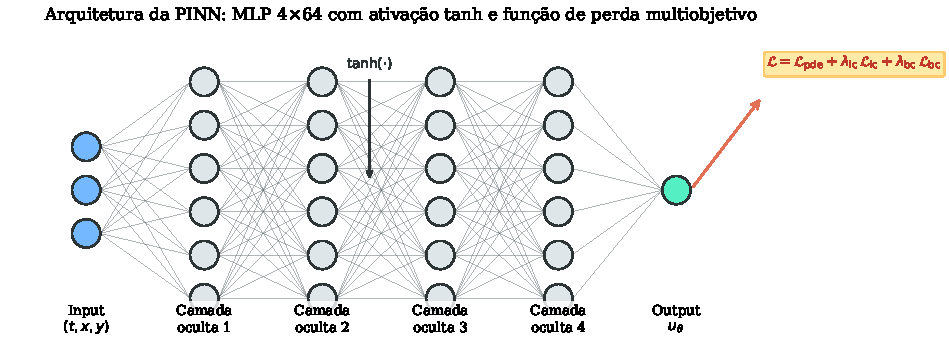
\includegraphics[width=0.64\textwidth]{figures/pinn_architecture.pdf}\\
{\footnotesize Fonte: Elaboração própria.}
\end{figure}

\textbf{3. Arquitetura Neural, Autograd e Retropropagação:} A aproximação contínua $\mathbf{u}_\theta(\mathbf{z})$ com entrada $\mathbf{z} = [x, y, t]^\top \in \mathbb{R}^3$ é modelada por uma MLP de $L=4$ camadas ocultas com $d_h=64$ neurônios (Figura~\ref{fig:arch}): $\mathbf{h}^{(1)} = \sigma(\mathbf{W}^{(1)}\mathbf{z} + \mathbf{b}^{(1)})$, $\mathbf{h}^{(\ell)} = \sigma(\mathbf{W}^{(\ell)}\mathbf{h}^{(\ell-1)} + \mathbf{b}^{(\ell)})$, $\mathbf{u}_\theta = \mathbf{W}^{(L+1)}\mathbf{h}^{(L)} + \mathbf{b}^{(L+1)}$, com ativação suave $\sigma(s) = \tanh(s) \in C^\infty(\mathbb{R})$. O treinamento articula um duplo fluxo de gradientes: (i) a \textbf{diferenciação automática (\textit{autograd})} em relação a $\mathbf{z}$ avalia exatamente as derivadas parciais da EDP via produtos vetor-Jacobiano (VJP): $\frac{\partial \mathbf{u}_\theta}{\partial x_j} = \nabla_{\mathbf{z}}\mathbf{u}_\theta \cdot \mathbf{e}_j$ e $\frac{\partial^2 \mathbf{u}_\theta}{\partial x_j^2} = \nabla_{\mathbf{z}}(\frac{\partial \mathbf{u}_\theta}{\partial x_j}) \cdot \mathbf{e}_j$; e (ii) o algoritmo de \textbf{retropropagação (\textit{backpropagation})} propaga o resíduo do funcional $\mathcal{L}(\theta)$ pelas camadas para computar $\nabla_\theta \mathcal{L}(\theta)$ e atualizar os pesos sinápticos via otimização estocástica.

\subsection{Metodologia}

A otimização minimiza os parâmetros $\theta$ sob o funcional multiobjetivo ponderado $L_2$:
\begin{equation}
    \mathcal{L}(\theta) = \lambda_{\mathrm{pde}}\mathcal{L}_{\mathrm{pde}}(\theta) + \lambda_{\mathrm{ic}}\mathcal{L}_{\mathrm{ic}}(\theta) + \lambda_{\mathrm{bc}}\mathcal{L}_{\mathrm{bc}}(\theta), \label{eq:loss}
\end{equation}
com $\mathcal{L}_{\mathrm{pde}} = \frac{1}{N_f}\sum \|\mathcal{R}[\mathbf{u}_\theta]\|_2^2$, $\mathcal{L}_{\mathrm{ic}} = \frac{1}{N_0}\sum \|\mathbf{u}_\theta - \mathbf{u}_0\|_2^2$, $\mathcal{L}_{\mathrm{bc}} = \frac{1}{N_b}\sum \|\mathbf{u}_\theta - \mathbf{g}\|_2^2$ e $\lambda_{\mathrm{pde}} = \lambda_{\mathrm{ic}} = \lambda_{\mathrm{bc}} = 1{,}0$. A Tabela~\ref{tab:config} sumariza os parâmetros experimentais adotados no treinamento ($20.000$ épocas Adam com $\eta = 10^{-3}$).

\begin{table}[!ht]
\centering
\caption{Parâmetros experimentais e hiperparâmetros de rede para Calor 2D e Burgers 2D.}
\label{tab:config}
\footnotesize
\setlength{\tabcolsep}{4.5pt}
\begin{tabular}{lcc}
\toprule
\textbf{Hiperparâmetro / Configuração} & \textbf{Equação do Calor 2D} & \textbf{Equação de Burgers 2D} \\
\midrule
Arquitetura Neural & MLP ($4 \times 64$, $\tanh$) & MLP ($4 \times 64$, $\tanh$) \\
Dimensão Entrada / Saída & $(x, y, t) \in \mathbb{R}^3 \to u \in \mathbb{R}$ & $(x, y, t) \in \mathbb{R}^3 \to (u, v) \in \mathbb{R}^2$ \\
Parâmetros Treináveis ($N_\theta$) & $12.865$ & $12.930$ \\
Pontos de Colocação ($N_f / N_0 / N_b$) & $10.000 \;/\; 10.000 \;/\; 4.000$ & $10.000 \;/\; 10.000 \;/\; 4.000$ \\
Parâmetro Físico Fundamental & $\alpha = 0{,}1\,\text{m}^2/\text{s}$ & $\nu = 0{,}01\,\text{m}^2/\text{s}$ \\
Domínio Espaço-Temporal & $[0, 1]^2 \times [0, 1{,}0]\,\text{s}$ & $[-1, 1]^2 \times [0, 1{,}0]\,\text{s}$ \\
Condição de Contorno & Dirichlet $u|_{\partial\Omega} = 1{,}0$ & Dirichlet $\mathbf{u}|_{\partial\Omega} = \mathbf{0}$ \\
Otimizador e Épocas & Adam ($\eta = 10^{-3}$, $20.000$ épocas) & Adam ($\eta = 10^{-3}$, $20.000$ épocas) \\
\bottomrule
\end{tabular}
\caption*{Fonte: Elaboração própria.}
\end{table}

\subsection{Resultados e Discussão}

\textbf{Dinâmica de Convergência das Perdas:} A trajetória das componentes de perda ao longo das $20.000$ iterações é apresentada na Figura~\ref{fig:loss}. No problema do calor (Figura~\ref{fig:loss}(a)), a linearidade assegura rápido decaimento assintótico, atingindo $\mathcal{L}_{\mathrm{total}} = 7{,}95 \times 10^{-5}$ com resíduo da EDP $\mathcal{L}_{\mathrm{pde}} = 6{,}47 \times 10^{-5}$. Em Burgers (Figura~\ref{fig:loss}(b)), as bordas homogêneas viabilizam $\mathcal{L}_{\mathrm{bc}} = 2{,}31 \times 10^{-6}$ e resíduo total $\mathcal{L}_{\mathrm{total}} = 1{,}04 \times 10^{-3}$, confirmando o ajuste estrito das restrições físicas.

\begin{figure}[!ht]
\centering
\caption{Curvas de convergência semilogarítmica do treinamento da PINN ao longo de 20.000 épocas: (a) Equação do Calor 2D ($\alpha = 0{,}1\,\mathrm{m^2/s}$); e (b) Equação de Burgers 2D ($\nu = 0{,}01\,\mathrm{m^2/s}$).}
\label{fig:loss}
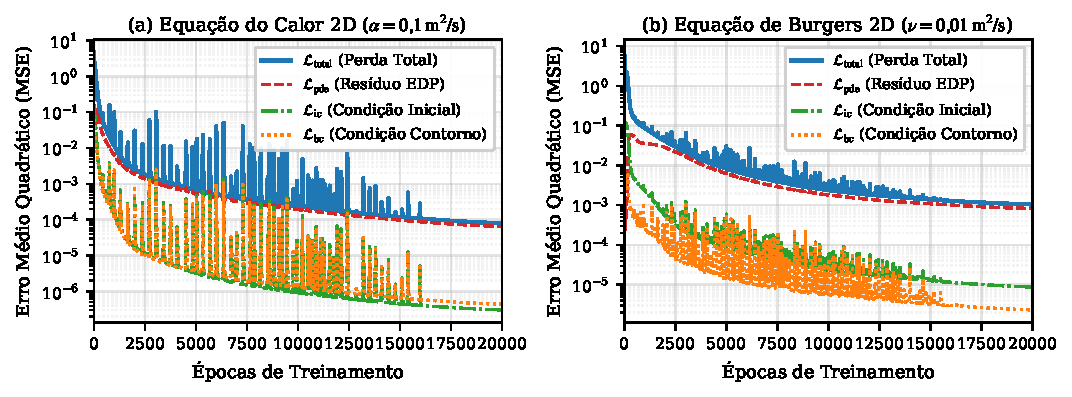
\includegraphics[width=0.92\textwidth]{figures/fig_loss_curves.pdf}\\
{\footnotesize Fonte: Elaboração própria.}
\end{figure}

\textbf{Experimento 1 --- Difusão Térmica 2D e Validação Analítica:} A Figura~\ref{fig:heat_3d} ilustra a evolução da superfície $u_\theta(x, y, t)$ em quatro instantes temporais. Em $t=0{,}0\,\text{s}$, a rede capta a base fria $u=0$ com contornos quentes $u=1$. Com o avanço do tempo ($t = 0{,}3 \to 0{,}7 \to 1{,}0\,\text{s}$), a difusão penetra homogeneamente ao centro. A validação frente à solução analítica em malha $100 \times 100$ comprova erro relativo $\epsilon_{L^2} = 1{,}40 \times 10^{-3}$ ($0{,}14\%$) e erro máximo $\epsilon_{L^\infty} = 1{,}29 \times 10^{-3}$.

\begin{figure}[!ht]
\centering
\caption{Equação do Calor 2D: evolução da distribuição de temperatura em superfície tridimensional $u_\theta(x,y,t)$ predita pela PINN para $t \in \{0{,}0;\, 0{,}3;\, 0{,}7;\, 1{,}0\}\,\mathrm{s}$ ($\alpha = 0{,}1\,\mathrm{m^2/s}$).}
\label{fig:heat_3d}
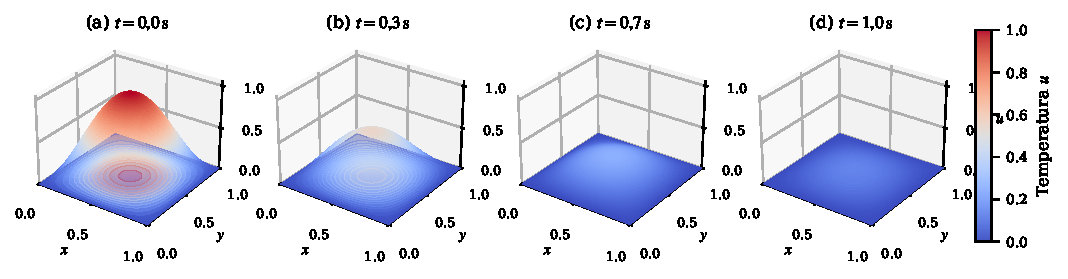
\includegraphics[width=0.88\textwidth]{figures/fig_h3_heat_3d_large.pdf}\\
{\footnotesize Fonte: Elaboração própria.}
\end{figure}

\textbf{Experimento 2 --- Dinâmica Não Linear dos Vórtices de Burgers 2D:} A Figura~\ref{fig:burgers} exibe a interação advectivo-difusiva da estrutura quadrupolar. Em $t=0{,}0\,\text{s}$ (Figura~\ref{fig:burgers}(a)), o campo de magnitude $\|\mathbf{u}\| = \sqrt{u^2 + v^2}$ revela quatro lóbulos simétricos de velocidade concentrados em $(\pm 0{,}3,\, 0)$ e $(0,\, \pm 0{,}3)$ com $\|\mathbf{u}\| \approx 1{,}0\,\text{m/s}$, direcionados simultaneamente para a origem. Em $t=0{,}3\,\text{s}$ (Figura~\ref{fig:burgers}(b)), a advecção não linear $(\mathbf{u}\cdot\nabla)\mathbf{u}$ atrai os quatro núcleos, deflagrando uma frente de colisão central em cruz com gradientes pronunciados. Em $t=0{,}5\,\text{s}$ (Figura~\ref{fig:burgers}(c)), ocorre a coalescência dos vórtices sob forte cisalhamento e rotação local. Em $t=1{,}0\,\text{s}$ (Figura~\ref{fig:burgers}(d)), a dissipação viscosa ($\nu = 0{,}01\,\text{m}^2/\text{s}$) amortece o fluxo para $\|\mathbf{u}\| \approx 0{,}18\,\text{m/s}$ sem gerar instabilidades numéricas.

\textbf{Análise Comparativa e Desempenho Computacional:} A Tabela~\ref{tab:comparison} consolida os resultados quantitativos. Enquanto esquemas clássicos de diferenças finitas investigados por \textcite{pereira2019} impõem avanços passo a passo com restrições de estabilidade CFL e interpolações nodais que degradam gradientes íngremes, a PINN resolve todo o bloco espaço-temporal $\Omega \times [0, T]$ em um bloco unificado. Uma vez ajustados os tensores $\theta$, a avaliação contínua para $10.000$ coordenadas arbitrárias em GPU requer meros $1{,}09\,\text{ms}$ no calor e $2{,}45\,\text{ms}$ em Burgers. A ativação $\tanh \in C^\infty$ permite extrair instantaneamente grandezas derivadas exatas via autograd (como fluxos térmicos $\mathbf{q} = -\kappa \nabla u$, vorticidade $\omega = \frac{\partial v}{\partial x} - \frac{\partial u}{\partial y}$ e dissipação viscosa $\varepsilon = \nu \|\nabla \mathbf{u}\|^2$) sem aproximações numéricas adicionais.

\begin{figure}[!ht]
\centering
\caption{Equação de Burgers 2D. (a,b): mapa de calor da norma da velocidade $\|\mathbf{u}\|$ em $t=0{,}0$ e $t=0{,}5$. (c,d): superfície tridimensional da componente de velocidade $u(x,y,t)$ em $t=0{,}0$ e $t=0{,}5$.}
\label{fig:burgers}
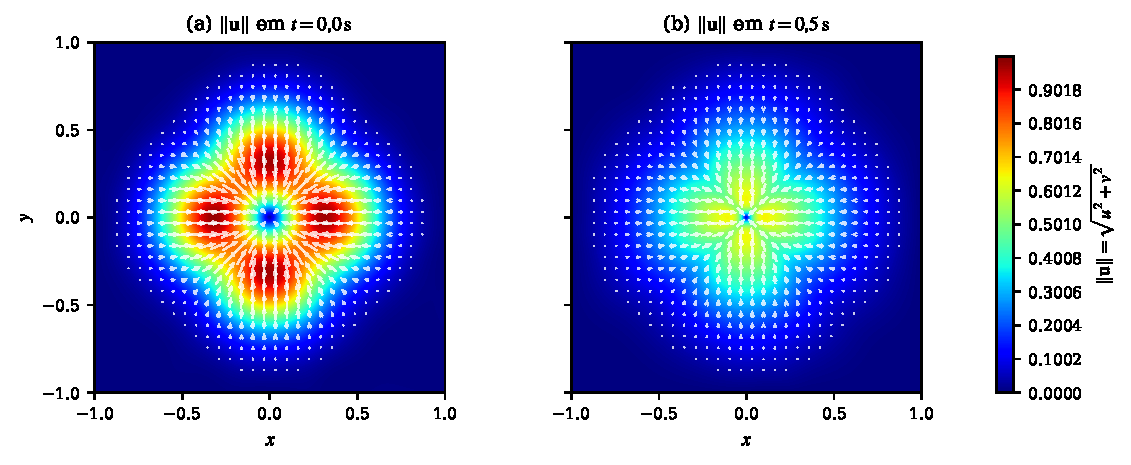
\includegraphics[width=0.48\textwidth]{figures/fig_b_burgers_2d_norm.pdf}
\hfill
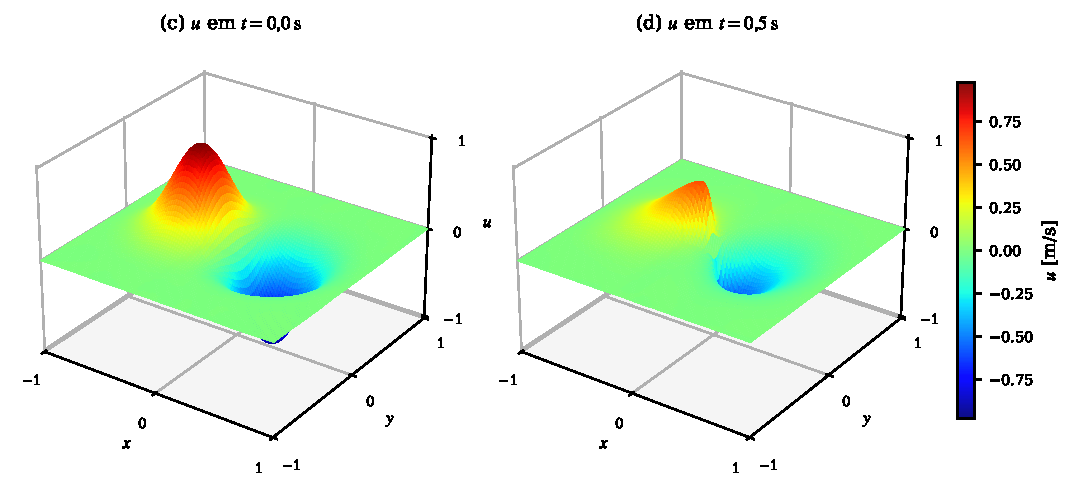
\includegraphics[width=0.48\textwidth]{figures/fig_b_burgers_3d_u.pdf}\\
{\footnotesize Fonte: Elaboração própria.}
\end{figure}

\begin{table}[!ht]
\centering
\caption{Síntese dos indicadores quantitativos de convergência e desempenho das PINNs.}
\label{tab:comparison}
\footnotesize
\setlength{\tabcolsep}{3.5pt}
\begin{tabular}{lcc}
\toprule
\textbf{Indicador Quantitativo de Desempenho} & \textbf{Calor 2D ($\alpha = 0{,}1$)} & \textbf{Burgers 2D ($\nu = 0{,}01$)} \\
\midrule
Perda Total Final ($\mathcal{L}_{\mathrm{total}}$) & $7{,}95 \times 10^{-5}$ & $1{,}04 \times 10^{-3}$ \\
Resíduo da EDP ($\mathcal{L}_{\mathrm{pde}}$) & $6{,}47 \times 10^{-5}$ & $8{,}23 \times 10^{-4}$ \\
Resíduo de Contorno ($\mathcal{L}_{\mathrm{bc}}$) & $4{,}36 \times 10^{-7}$ & $2{,}31 \times 10^{-6}$ \\
Resíduo de Condição Inicial ($\mathcal{L}_{\mathrm{ic}}$) & $3{,}04 \times 10^{-7}$ & $8{,}71 \times 10^{-6}$ \\
Erro Relativo ($\epsilon_{L^2}$) & $1{,}40 \times 10^{-3}$ ($0{,}14\%$) & --- \\
Erro Máximo ($\epsilon_{L^\infty}$) & $1{,}29 \times 10^{-3}$ & --- \\
Tempo de Inferência ($10^4$ pontos) & $1{,}09\,\text{ms}$ & $2{,}45\,\text{ms}$ \\
Parâmetros / Tamanho do Modelo & $12.865$ ($198\,\text{kB}$) & $12.930$ ($202\,\text{kB}$) \\
\bottomrule
\end{tabular}
\caption*{Fonte: Elaboração própria.}
\end{table}

\section{Considerações Finais}

Os resultados comprovam que as Redes Neurais Informadas por Física constituem uma metodologia precisa, compacta e eficiente para a resolução de EDPs lineares parabólicas (Calor 2D) e sistemas acoplados fortemente não lineares (Burgers 2D). A sinergia entre o cálculo exato de operadores diferenciais via autograd e a retropropagação (\textit{backpropagation}) do funcional multiobjetivo supera os gargalos clássicos de discretização do MDF formalizados por \textcite{pereira2019}. A validação analítica comprova erro relativo inferior a $0{,}15\%$, enquanto o experimento de Burgers confirma a captura estável da dinâmica de colisão quadrupolar e amortecimento viscoso sustentada por perdas residuais $\mathcal{L}_{\mathrm{total}} \sim 10^{-3}$. O custo inicial de treinamento em GPU é amplamente amortizado pela inferência ultrarrápida em escala de milissegundos ($\sim 1 \dots 2{,}5\,\text{ms}$). Trabalhos futuros incluem problemas inversos de estimação paramétrica e escoamentos turbulentos 3D.

\renewcommand*{\bibfont}{\small}
\setlength{\bibitemsep}{2pt}
\begin{refcontext}[sorting=none]
\printbibliography
\end{refcontext}

\end{document}

